% !TEX root = ../my-thesis.tex
%
\selectlanguage{english}  
\chapter{\textcolor{ctcolormain}{Carbon sequestration of coppiced forests of \Qp. An study case from the rear-edge of its distribution}}\label{sec:carbon}

\mbox{}
\vfill
{\color{ctcolormain}\textbf{Antonio J. Pérez-Luque}}; Mihai Tanase; Cristina Aponte \& Regino Zamora (In prep.)


\newpage

\paragraph{Abstract} \mbox{} \\

\newpage

\section{Introduction}\label{sec:carbon:intro}

Forest ecosystems are suppliers of several ecosystems services to humans \autocite{Iversonetal2018EcosystemServices,MartinezPasturetal2018EcosystemServices,NoceSantini2018MediterraneanForest}. Forest ecosystem services include provisioning services (\emph{e.g.} wood and non-wood forest products), regulating services (\emph{e.g.} climate regulation), habitat or support services, and cultural services. In Mediterranean region, humans have been exploiting forest resources for centuries \autocite{ValbuenaCarabanaetal2010HistoricalRecent}, however in the last decades a strong abandonment of traditional activities in mountains regions have been observed, mainly due to the rural exodus and the low economic value of forest products activities \autocite{Chauchardetal2007PatternsLanduse,Debusscheetal1999MediterraneanLandscape,MacDonaldetal2000AgriculturalAbandonment}. As a result, many forests currently have high tree-density stands, with an increased competition for resources, which can lead to widespread weakening of stand, increasing the vulnerability of forests to abiotic and biotic disturbances \autocite{Tardieuetal2018HumanNeeds}. This may be especially relevant for forests stands located at the rear-edge of the species distribution \autocite{HampePetit2005ConservingBiodiversity}, which are usually considered more vulnerable to climate change compared with populations at the centre of a species' range \autocite{Fadyetal2016EvolutionbasedApproach,Pirononetal2017GeographicVariation,Rehmetal2015LosingYour}.

\Qp (Pyrenean oak) is a marcescent Mediterranean tree species widely distributed throughout southwestern France and the Iberian Peninsula, reaching their southern limit in mountain areas of northern Morocco \autocite{Franco1990Quercus}. The rear-edge populations of this species are restricted to high-mountain areas where these populations persists as isolated nuclei with ecological conditions very different from those of the main distribution area \autocite{PerezLuqueetal2021EcologicalDiversity}. Due to its ability to resprout from stumps and the entire root system, most stands of this species have been coppiced for centuries mainly for firewood, charcoal, tannins and woody pasture production \autocite{SanchezPalomaresetal2008EstacionesEcologicas,XimenezdeEmbun1961MonteBajo}. All these anthropogenic processes have transformed native woodland structures \autocite{Tarregaetal2006ForestStructure}, and nowadays it is difficult to find stands of this oak that can be qualified as natural or pristine forests \autocite{RuizdelaTorre2006FloraMayor}. Paradoxically, after the diminution of human pressure on woodlands over the last decades, the abandonded coppices of \Qp present an advanced state of degradation with important ecological, economic and social problems \autocite{Bravoetal2008SelviculturaMontes,MontoyaMeson1979SituacionActual,Piqueetal2018Spain,PiqueVericat2015EvolutionPerspectives,Vericatetal2012GestionAdaptativa}. Due to the importance of this species, several management practices (\emph{e.g.}~conversion to high forest) have been proposed to improve the state of abandoned coppices \autocite{Bravoetal2008SelviculturaMontes,Montoya1982SelviculturaOrdenacion,Montoya1983UsosAlternativos,Serradaetal1992CoppiceSystem,Vericatetal2012GestionAdaptativa}, although they have not been very successful, partly due to the lack of a comprehensive understanding of the physiological mechanisms underpinning tree stagnation \autocite{Salomonetal2017GeneralFailure,ValbuenaCarabanaGil2017CentenaryCoppicing}. In view of this situation, it is essential to seek for alternative management practices to the traditional uses of the abandoned coppices \autocite{MesonMontoya1985VegetacionForestal,SanMigueletal2012BosquesMatorrales}. Some management alternatives based on pastoral use have been proposed \autocite{HerreraCalvo2016UsoPastoral}, but to our knowledge few proposals have focused on the provision of the ecosystem services provided by this oak forests \autocites[but see][]{Piqueetal2018Spain,PiqueVericat2015EvolutionPerspectives}.

The carbon sequestration is one of the most relevant ecosystems services provided by Mediterranean forests \autocite{Gauquelinetal2018MediterraneanForests,NoceSantini2018MediterraneanForest}. Carbon stock can be assumed as an indicator of the capacity of ecosystems to contribute to climate regulation because their potential to influence atmospheric CO\textsubscript{2} concentration \autocite{Lauterbach2007AssessmentExisting,Luyssaertetal2008OldgrowthForests}. Mediterranean forests represent a carbon sink expected to increase over coming decades \autocite{Canellasetal2017CarbonSequestration,PasalodosTatoetal2017EvaluationTree}. Improving carbon estimation and our understanding of the effects of forest management could be useful for forest managers, which could include carbon sequestration among the different objectives pursued in the forests management \autocite{RuizPeinadoetal2017ForestManagement}. Several studies have been conducted to determine carbon sequestration by forest ecosystems in the Mediterranean region based on data from forest carbon inventories, field measurements, remote sensing, laser scanning and growth simulation \autocites[\emph{e.g.}][]{Canellasetal2008SilvicultureCarbon,Chiesietal2005ModellingCarbon,Garciaetal2010EstimatingBiomass,GuerraHernandezetal2016ComparisonALS,Simonsonetal2016ModellingAboveground,Vayredaetal2012SpatialPatterns}. LIDAR (Light Detection And Ranging) has emerged as an effective technique for quantifying aboveground biomass in forests \autocite{Belandetal2019PromotingUse,Lefskyetal2002LidarRemote,Xiaoetal2019RemoteSensing} and has been also used for quantifying carbon stocks \autocite{Simonsonetal2016ModellingAboveground,Zhaoetal2018UtilityMultitemporal}. In this study we combined Airborne Laser Scanning LIDAR data and field inventories to estimate the biomass of Pyrenean oak woodlands (\Qp) of Sierra Nevada (southern Spain), and then to assess the carbon sequestration capacity of those forests and their role as carbon sink. The specific objectives are: \emph{(i)} to estimate the potential capacity of these ecosystems to sequester carbon dioxide and to evaluate the temporal trends for this ecosystem service; \emph{(ii)} to explore the factors that explain the C stock for \Qp woodland in Sierra Nevada; and \emph{(ii)} to analyse the differences in biomass and carbon sequestration among oak populations within this mountain region.  

\section{Material and Methods}\label{sec:carbon:mat}
\subsection{Study site and oak woodlands}\label{sec:carbon:mat-studysite}
The study area is located in Sierra Nevada (37°N, 3°W), a high-mountain range of southern of Andalusia with elevations of up to 3 482 \eleven. The climate is Mediterranean, characterized by cold winters and hot summers, with pronounced summer drought and increasing aridity with decreasing altitude, and marked variability according to elevation and aspect. In Sierra Nevada there are eight Pyrenean oak populations (2 400 ha), distributed from 1 100 to 2 000 \eleven and often associated with major river valleys. Those eight oak populations could be grouped in three clusters, based on their structure and floristic composition: the northern (N), the northwestern (NW), and the southern (S) clusters \autocite[see chapter \ref{sec:multivar}; also][]{PerezLuqueetal2021EcologicalDiversity}. \Qp woodlands in this mountain region represent a rear edge of their habitat distribution \autocite{HampePetit2005ConservingBiodiversity}. They are the richest forest formation in vascular plant species of Sierra Nevada, containing several endemic and endangered plant species \autocite{Loriteetal2008PhytosociologicalReview}, and they also harbor high levels of intraspecific genetic diversity \autocite{ValbuenaCarabanaGil2013GeneticResilience}. However, these relict forests have undergone intensive human use throughout history \autocite{CamachoOlmedoetal2002DinamicaEvolutiva}. Furthermore, the conservation status of this species for southern Spain is considered \emph{"Vulnerable"} and it is expected to suffer from climate change, reducing its suitable habitats in the near future \autocite{GeaIzquierdoetal2013GrowthProjections,GeaIzquierdoetal2017RiskyFuture,Benitoetal2011SimulatingPotential}.

\begin{table}[]
\caption{Allometric equations to compute biomass fraction of \Qp \autocite{RuizPeinadoetal2012BiomassModels}. DBH: Diameter at breast height; h: Tree height.}
\label{tab:carbon:biomasseq}
\resizebox{\textwidth}{!}{%
\begin{tabular}{@{}ll@{}}
\toprule
Tree fraction & Equation \\ \midrule
Stem and thick branches  & \textbf{\ws} = 0.0261 DBH\textsuperscript{2} \\
Medium branches & \textbf{\wbs} = \textendash0.0260 DBH\textsuperscript{2} + 0.536 h + 0.00538 DBH\textsuperscript{2} h \\
Thin branches and leaves & \textbf{\wb} = 0.898 DBH \textendash0.445 h \\
Roots & \textbf{\wro} = 0.143 DBH\textsuperscript{2} \\ \bottomrule
\end{tabular}%
}
\end{table}


\subsection{Biomass data}\label{sec:carbon:mat-field-data}

We used two types of field data, inventories (previous collected, xx plots), and field data (xx plots) collected for this study. 

\begin{sidewaystable} 
\caption{Field data used to compute the biomass of \Qp. For DBH (Diameter at breast height) and Tree height, the average values and range (in brackets) are shown.}\label{tab:carbon:inventories}
\begin{adjustbox}{width=\linewidth}
	\begin{threeparttable}
		\begin{tabular}{p{10cm}lllllll}
		\toprule[0.5pt]
		\textbf{Source} & \textbf{n plots} & \textbf{area (m\textsuperscript{2})} & \textbf{year} & \textbf{\# trees} & \textbf{DBH (cm)} & \textbf{Tree height (m)} \\ \toprule 
		Dataset of Global Change, altitudinal range shift and colonization of degraded habitats in Mediterranean mountains (MIGRAME) \autocite{PerezLuqueetal2015DatasetMIGRAME} & 30 & 300 & 2012 & 1422 & 10.77 (7.5--105) & 4.27 (1.1--18) \\ \midrule
		Sierra Nevada Global Change Observatory \autocites{Aspizuaetal2014EvaluacionGestion,Zamoraetal2017GlobalChange} & 3 & 400 & 2011,2012 & 122 & 19.03 (8--36) & 9.57 (4.7--16.4) \\ \midrule
		Protection of key ecosystem services by adaptive management of climate change endangered mediterranean socioecosystems \autocite{BareaAzconetal2017LIFEADAPTAMED}. Forest inventories from Action C6 of the project & 16 & 706.85 & 2015, 2017 & 650 & 13.26 (7.6--50) & 6.96 (3.6--14) \\ \midrule
		Protection of key ecosystem services by adaptive management of climate change endangered mediterranean socioecosystems \autocite{BareaAzconetal2017LIFEADAPTAMED}. Forest inventories associated with dendrochronological plots & 2 & 254.47--530.93 & 2018 & 191 & 7.73 (2.1--42.2) & 4.48 (1.1--13.6) \\ \midrule
		Forest inventories from dendroecological research \autocite[see chapter \ref{sec:dendro};][]{PerezLuqueetal2020LanduseLegacies} & 39 & 314.16 & 2018 & 457 & 26.3 (2.86--122.55) & 10.31 (3--20.4) \\ \midrule
		This study field data & 23 & 254.47--706.85 & 2019,2020 & 382 & 24.32 (2.91--67) & 11.42 (1.7--20.6) \\ \bottomrule
		\end{tabular}
	\end{threeparttable}
\end{adjustbox}
\end{sidewaystable}

Field data were obtained from a compilation of several forest inventories carried out in the Sierra Nevada mountain range (\tabref{tab:carbon:inventories}). In a first step, we selected plots included in the current distribution of Pyrenean oak in Sierra Nevada \autocite{PerezLuqueetal2019MapEcosystems}. Then, only plots with complete information (\emph{i.e.} those where all tree individual with dbh \textgreater{} 7.5 cm were measured), and pure stands (\emph{i.e.} \Qp composition \textgreater{} 70\%) were selected. A spatial filter was also applied to discard overlapping plots. We also discarded old forests inventories (\emph{i.e.} more than 10 years). All selected plots were measured between 2012 and 2020. In order to have a representation of all the oak populations, additional circular plots (radius 9 to 16 m) were sampled between October 2019 and March 2020. The plots were selected in proportion to the extension of the different ecological strata, providing representative stands with a variety of stand structure and site conditions. A sub-meter global satellite receiver (Leica Zeno 20 GIS, Leica Geosystems, Switzerland) was used to survey plot centers. We tagged and measured all tree individuals within the circular plot. Diameter at breast height (DBH) was measured to the nearest 0.1 cm with a graduated caliper, and tree height was measured to the nearest 0.1 m with a hypsometer. Azimuth and distance of each measured tree from the plot center were also recorded. A total of 113 plots (254 to 400 m\^{}2) were finally selected with a total of 3 224 measured trees (\tabref{tab:carbon:inventories}).

\subsection{Biomass and Carbon estimation}\label{sec:carbon:mat-biomass}

The biomass of individual trees was estimated according to published species-specific allometric equations \autocite{RuizPeinadoetal2012BiomassModels}. For each tree, dry biomass was estimated as a sum of the different fractions \autocite{CarvalhoParresol2003AdditivityTree}: stem plus branches with a diameter \textgreater{} 7 cm (\ws); branches with a diameter between 2 and 7 cm (\wbs), branches with a diameter of less than 2 cm with leaves (\wb), and the belowground fraction (\wro) the roots. Biomass of each fraction were computed using the equations developed for \Qp \autocite{RuizPeinadoetal2012BiomassModels} (\tabref{tab:carbon:biomasseq}).

The carbon content in each biomass fraction was calculated by multiplying each value by 0.475, \emph{i.e.} the species-specific carbon content of the biomass for this species  \autocite{Ibanezetal2002MetodologiaComplementaria,Monteroetal2005ProduccionBiomasa}. The equivalent tree CO\textsubscript{2} sequestration was estimated by multiplying the tree carbon content by 3.67, \emph{i.e.} the ratio between CO\textsubscript{2} molecular weight and C atomic weight. Biomass and carbon storage of individual trees were aggregated at plot level and  scaled-up to hectarea to obtain the values of biomass for each fraction (\mgha), and the total carbon storage (\mgha) at the plot level.

\subsection{Airborne Laser Scanning (ALS) Data and processing}\label{sec:carbon:mat-lidar}
Airborne Laser Scanning (ALS) data were acquired in 2014, with up to four returns measured per pulse, within the Spanish National Plan for Aerial Orthophotography (PNOA, by its Spanish language acronym) were used to generate the biomass map. The nominal point density was 0.5 points m$^-2$ with a vertical accuracy better than 0.20 m. 
The data were examined for extent, point density and consistency with overlapping points from adjacent scanning lines being removed. Gap filling was carried out when data from additional flight lines were available. The point clouds were classified into ground and non-ground using the Multiscale Curvature Classification (MCC) algorithm \autocite{EvansHudak2007MultiscaleCurvature}. Non-ground returns were labelled as vegetation as no infrastructure is present in the study area. The classified point cloud (ground class) was used to derive a digital elevation model (DEM). The DEM was subsequently used to compute the height above ground (\emph{i.e.} normalized height) for the points classified as vegetation. Based on the height above ground, four generic groups of lidar metrics were generated at 20-m spatial resolution: canopy metrics, strata metrics, first returns metrics and all returns metrics. For example, canopy metrics included canopy closure at different heights (\emph{i.e.}, 1-, 2-, 4-, 6-, 8-, 10-, and 12-m) while strata metrics included canopy closure and forest density for specific strata (\emph{i.e.}, 0-0.5 m, 1-6 m, 1-8 m, 1-10 m, 1-12 m, 1-16 m, 1-24 m, 2-4 m, 2-6 m,..., 8-16 m, 8-24 m). Percentiles were computed using first returns as well as all returns metrics. Canopy closure metrics were defined as the proportion of first returns over a specific height threshold. Strata-specific canopy closure and forest density metrics were defined as the proportion of first returns and, respectively, all returns falling within specific height thresholds. Such metrics, representing proxies of forest structural characteristics, were aggregated at plot level and correlated with field-based plot biomass estimates to select optimum predictor variables for forest biomass.
A two-step variable selection approach was used to identify the best lidar predictors for each biomass fraction.  First, correlation among all 250 lidar variables was assessed and highly correlated (|r| > 0.7) variables were excluded from the dataset after retaining those with the highest correlation with biomass response variables (\ws, \wb, \wbs, \wro, and \wt). Second, the VSURF variable selection algorithm was implemented in R \autocite{VSURF} to identify the best predictors for each response variable. Briefly, this algorithm computes random forest models and variables are selected based on their importance value and on their capacity to decrease the OOB (out-of-bag) error of these models \autocite[more details can be found in VSURF package description, see][]{VSURF}. 

Biomass maps were generated based on the selected predictor lidar variables using a Support Vector Machines (SVM) classification. The SVM model's stability and error were computed by randomly splitting the dataset (\emph{n}=113 plots) into calibration and validation metrics (using a 60:40 rule). 100 random iterations were carried out to compute average error metrics including the average root mean squared error (RMSE), the relative RMSE (RMSE\%) and the correlation (r) between predicted and observed biomass. SVM biomass models were applied over the extents of the eight oak populations. For each biomass fraction, we compared the performance of the plot-scale biomass measurements (field data) with the predicted values derived from the ALS modelling. We used graphical methods and computed a Pearson correlation coefficient. 

\subsection{Cartography of biomass and C Stocks}\label{sec:carbon:mat-cmpas}
For each of the estimated biomass fractions obtained from the modelling, we generated a map of biomass and sequestered C for each of the oak populations studied. The distribution of \Qp forests in Sierra Nevada were obtained from vegetation and ecosystem maps of Sierra Nevada at 1:10 000 scale \autocite{CMAOT2014CartografiaEvaluacion,PerezLuqueetal2019MapEcosystems}. The pixel size selected to compute the ALS-derived metrics and to map the biomass and C stock was 20 m × 20 m, representing an area of 400 m\textsuperscript{2}, similar to the field plot dimensions (mean = 439 m\textsuperscript{2}, range 254 - 706.85) (\tabref{tab:carbon:inventories}).

\section{Temporal evolution of tree biomass in \Qp stands}\label{sec:carbon:mat-temporal}
We explored the temporal variation of biomass for this species at national level, and then only for plots located in our study area. To analyze the temporal evolution of the tree biomass of \Qp forests, we used data from Spanish National Forest Inventory (SNFI), an extensive national database of forest surveys distributed systematically across the forested area of Spain. We used data from the second \autocites[SNFI2,][]{VillaescusaDiaz1998SegundoInventario} and the third Spanish Forest Inventory \autocites[SNFI3,][]{Villanueva2005TercerInventario}, carried out during 1986-1996 and during 1997-2007, respectively. The SNFI is based on a network of circular plots which allows forest characterization and includes exhaustive information on the structure and composition of canopy and understory woody species. Each plot consisted of four concentric circles of \emph{radii} 5-, 10-, 15- and 25-m, in which DBH and total height were measured in all trees of DBH \textgreater{} 7.5-, 12.5-, 22.5- and 42.5-cm, respectively \autocite{Alberdietal2016SpanishNational}. Of the SNFI3 plots where \Qp was present (\emph{n} = 6382 plots), we selected only plots measured previously in the SNFI2, and with \Qp as the main dominant species (\emph{n} = 2269). For each plot, we computed aboveground and belowground biomass of each \Qp adult tree using allometric equations (\tabref{tab:carbon:biomasseq}) \autocite{RuizPeinadoetal2012BiomassModels}. We scaled-up to hectarea and aggregated at plot level. The temporal variation of biomass was estimated as the difference between biomass value of the same plot at the SNF3 and at the SNF2: \[\Delta Biomass = B_{i, SNFI3} - B_{i, SNFI2}\]

\section{Statistical analysis}\label{sec:carbon:analysis}
We analyzed differences of the ALS-derived biomass and carbon dioxide sequestration for each fraction among the different oak populations and oak-population clusters. Non parametric Kruskal-Wallis test were used because data do not fit normality, homocedasticity or independence. Multiple pairwise comparisons after this test were made using Dunn's test with Bonferroni's correction. We also explored differences in the forest structure among oak-populations clusters. For this purpose, we computed several forest attributes for each field plot: mean tree height (m), average DBH (cm), basal area (m\textsuperscript{2} ha\textsuperscript{-1}) and tree density (trees ha\textsuperscript{-1}). Differences for stand attributes among oak-population clusters were also analyzed with the non-parametric Kruskal-Wallis test, followed by multiple pairwise comparisons using Dunn's test with Bonferroni's correction. 

We used generalized linear models (GLM) to analyze the effect of the different explanatory variables and their interactions on the forest C stock (\emph{i.e.}: \wt, \ws, \wro). As explanatory variables we selected: topographic variables (elevation, slope and aspect); competition related-variables (tree density); stand-structural variables (Shannon structural diversity index and vertical strata richness); and microclimatic variables (topographic wetness index, a surrogate of the moisture content). Topographic variables were derived from a digital elevation model at 5 x 5 meters resolution (Spanish National Geographic Institute). For each plot we compute the tree density (trees ha\textsuperscript{-1}), and the strata richness (number of different diametric classes) using the DBH. We considered the following diametric classes: \textless2.5 cm; each 5 cm-intervals; and \textgreater52.5 cm. We also characterized the structural diversity by computing a Shannon-Weber structural diversity index following \autocite{delRioetal2003IndicesStand}. This index is considered a surrogate of structural heterogeneity \autocite{McElhinnyetal2005ForestWoodland,Gadowetal2012ForestStructure}. The topographic wetness index is an estimate of the predicted water accumulation and is considered a surrogate of soil-moisture \autocites[\emph{e.g.}][]{Zinkoetal2005PlantSpecies,Petrosellietal2013EcologicalBehavior}. It was derived from the high-resolution digital elevation model using the dynatopmodel R package \autocite{Metcalfeetal2018DynatopmodelImplementation}. Stepwise model selection was applied starting from the saturated model and removing the least significant term until there was no further decrease in the Bayesian Information Criterion (BIC). We considered all models within 2 BIC units as equivalent in terms of fit.

All analyses were conducted using the R software \autocite{base}, and the vegan \autocite{vegan}, randomForest \autocite{LiawWiener2002ClassificationRegression}, nlstools \autocite{nlstools}, nlme \autocite{nlme}, biostat \autocite{biostat}, glmulti \autocite{glmulti}, MuMIn \autocite{MuMIn} and VSURF packages \autocite{VSURF}. 

\section{Results}\label{sec:carbon:results}
\subsection{Biomass modelling}\label{sec:carbon:results-modelling}

The LIDAR-metrics that best predicted the each-fraction biomass values are presented in \tabref{tab:carbon:lidarmodels}. The rumple index, elevation, canopy height maximum and 99\textsuperscript{th} percentile of canopy height were the LIDAR-metrics better explained the biomass model for the \ws, \wbs and \wt fractions (\tabref{tab:carbon:lidarmodels}), and they also were selected in biomass model for the \wro and \wb fractions. The better models provided R\textsuperscript{2} values ranged from 0.17 (\wb) to 0.45 (\ws) (\tabref{tab:carbon:lidarmodels}).

The evaluation of the observed (field-measured) \emph{versus} the ALS-estimated values for all biomass fractions are presented in \figref{fig:carbon:compara}. The higher correlations were obtained for \ws and \wt fractions which showed 0.61 and 0.60 R\textsuperscript{2} values respectively. The other biomass components showed significant but weaker correlations, particularly the \wbs fraction with a R\textsuperscript{2} value of 0.14 (\figref{fig:carbon:compara}).

\begin{figure}
    \centering
    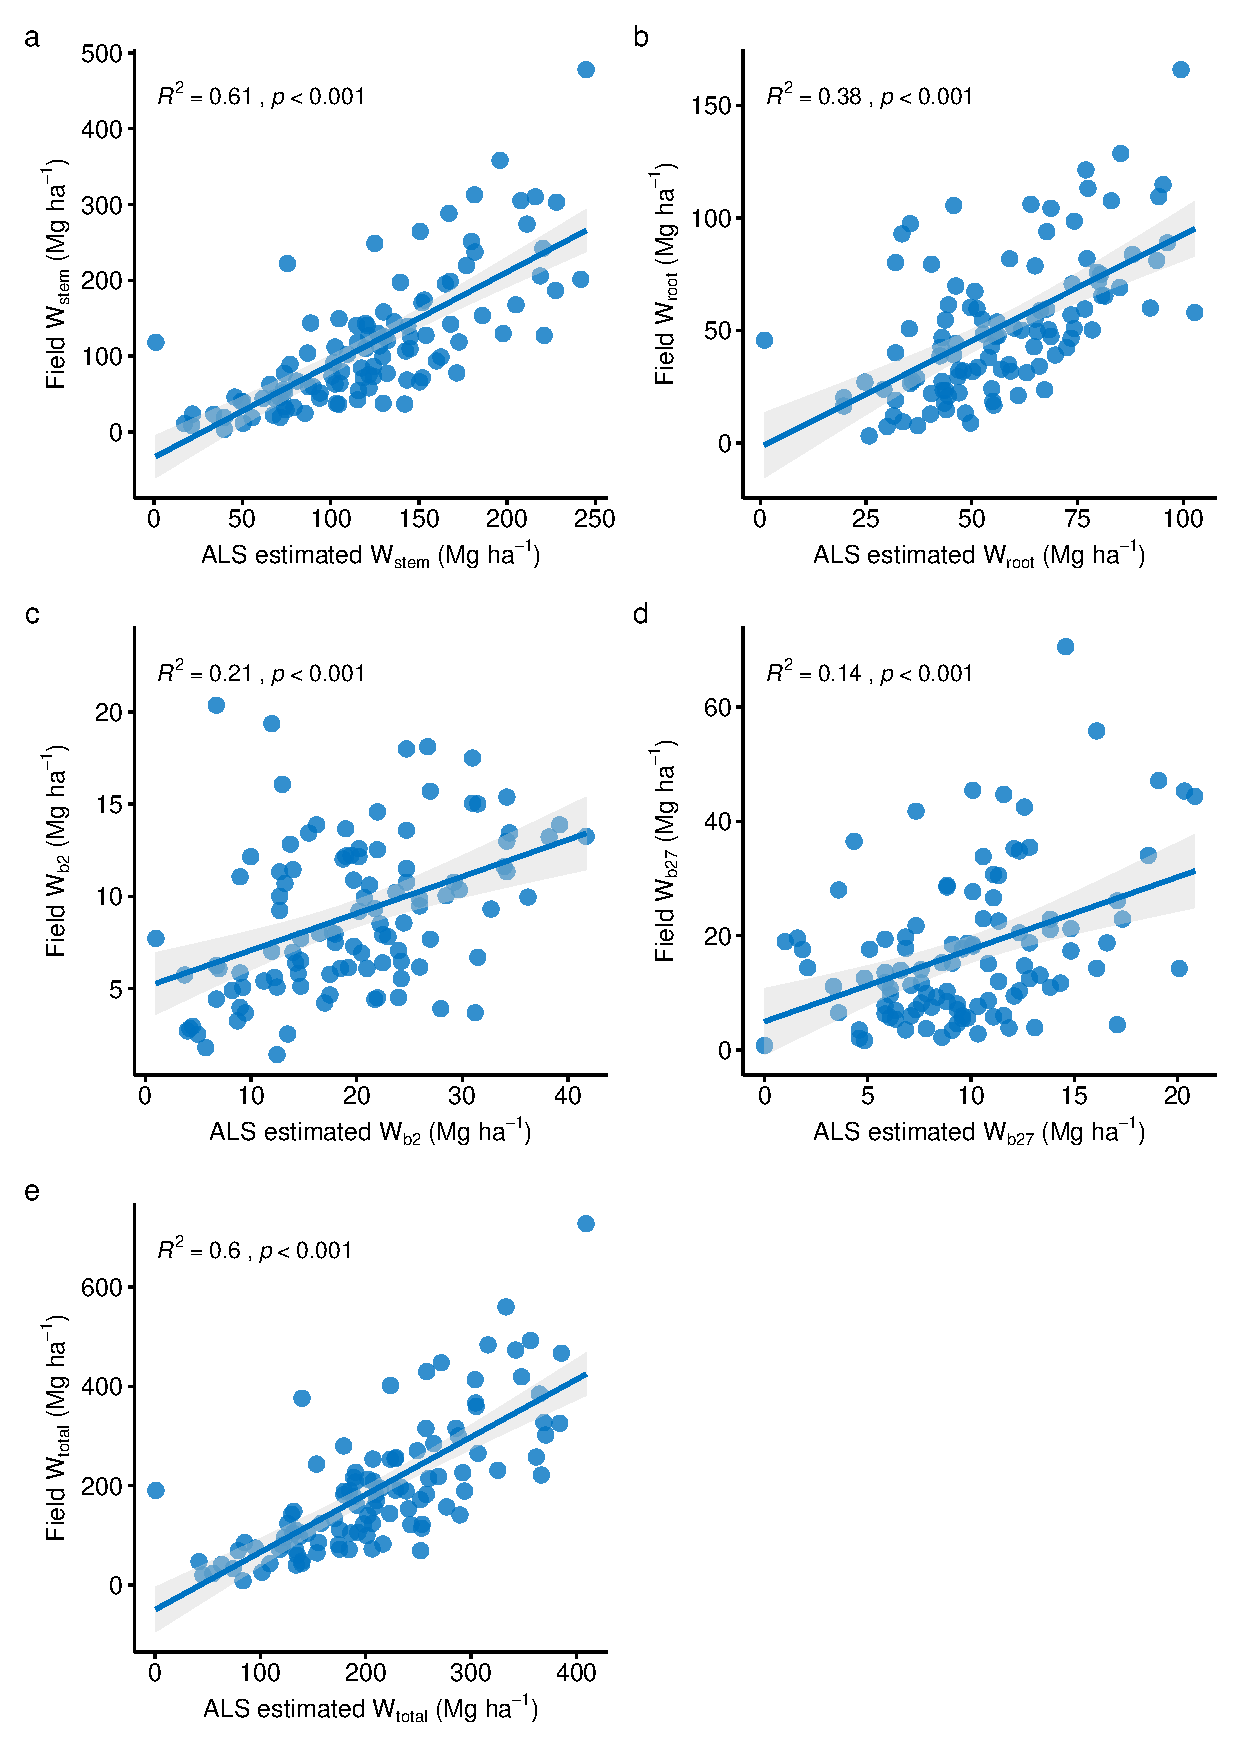
\includegraphics[height=.6\textheight]{img/carbon/carbon-compara-lidar-field.pdf}\caption{Scatterplots of the field-measured biomass fractions and the most accurate model-estimated values of the biomass fractions in the same plot. R\textsuperscript{2} and significance values of the correlation are included}\label{fig:carbon:compara}
\end{figure}

\begin{sidewaystable} 
\caption{Stand characteristics, field-measured and ALS-derived biomass (\mgha) and potential carbon dioxide sequestration (Mg CO$_2$ ha$^{-1}$) values for Pyrenean oak-population clusters in Sierra Nevada. Statistics and significance value for Kruskal-Wallis tests were shown. Different letters indicate statistically significant differences between oak-population clusters (Dunn's test, p < 0.05). Total values of ALS-derived Biomass (Mg) and Potential CO$_2$ sequestration (Mg CO$_2$) for all \Qp forests in Sierra Nevada are shown. Values in bracket show total values for each oak-population cluster.}\label{tab:carbon:compara}
\begin{adjustbox}{width=\linewidth}
	\begin{threeparttable}
		\begin{tabular}{lclclclrrr} 

\textbf{\emph{Stand features}} & \textbf{N} & ~ & \textbf{NW} & ~ & \textbf{S} & \textit{~} & \textit{Statistic} & \textit{p-value} &  \\ 
\toprule
Tree height (avg.) & 14.69 ± 0.81 a & ~ & 9.10 ± 0.55 b & ~ & 7.81 ± 0.36 b & ~ & 15.23 & \textit{\textless{}0.001} &  \\ 
Tree height (min) & 10.32 ± 1.49 a & ~ & 4.02 ± 0.52 b & ~ & 3.71 ± 0.31 b & ~ & 11.20 & \textit{0.004} &  \\ 
Tree height (max) & 18.54 ± 0.68 a & ~ & 14.76 ± 0.40 b & ~ & 13.89 ± 0.33 b & ~ & 12.67 & \textit{0.002} &  \\ 
DBH & 39.36 ± 6.00 a & ~ & 20.18 ± 1.24 b & ~ & 20.88 ± 1.54 b & ~ & 8.43 & 0.015 &  \\ 
Basal Area & 35.99 ± 6.61 a & ~ & 28.08 ± 2.34 a & ~ & 28.81 ± 2.26 a & ~ & 1.31 & 0.518 &  \\ 
Tree density & 405.51 ± 165.87 a & ~ & 898.86 ± 104.02 a & ~ & 838.35 ± 106.01 a & ~ & 3.69 & 0.158 &  \\ 
\midrule
\textbf{\emph{Field-measured biomass}} &  & ~ &  & ~ &  & ~ &  &  &  \\ 
\ws & 182.89 ± 33.18 & ~ & 113.21 ± 11.41 & ~ & 117.18 ± 11.72 & ~ & 4.30 & 0.116 &  \\ 
\wbs  & 28.82 ± 5.37 & ~ & 17.49 ± 1.85 & ~ & 17.31 ± 1.69 & ~ & 5.25 & 0.072 &  \\ 
\wb  & 8.75 ± 2.06 & ~ & 9.73 ± 0.74 & ~ & 8.63 ± 0.48 & ~ & 1.06 & 0.587 &  \\ 
\wro  & 65.52 ± 12.04 & ~ & 51.12 ± 4.26 & ~ & 52.46 ± 4.11 & ~ & 1.31 & 0.518 &  \\ 
\midrule
\textbf{\emph{ALS-derived measured}} &  & ~ &  & ~ &  & ~ &  &  & \textbf{\emph{Total}} \\ 
\ws & 84.29 ± 0.50 a (1.03 10$^6$) & ~ & 83.35 ± 0.37 a (1.98 10$^6$) & ~ & 89.16 ± 0.33 b (2.62 10$^6$) & ~ & 2296.42 & \textit{\textless{}0.001} & 5.62 10$^6$ \\
\wbs & 8.71 ± 0.04 a (0.10 10$^6$) & ~ & 8.24 ± 0.03 b (0.18 10$^6$) & ~ & 8.37 ± 0.02 c (0.24 10$^6$) & ~ & 1446.20 & \textit{\textless{}0.001} & 0.52 10$^6$ \\
\wb  & 13.16 ± 0.08 a (0.16 10$^6$) & ~ & 13.10 ± 0.06 a (0.31 10$^6$) & ~ & 14.18 ± 0.05 b (0.42 10$^6$) & ~ & 2138.11 & \textit{\textless{}0.001} & 0.89 10$^6$ \\
\wro  & 49.32 ± 0.21 a (0.59 10$^6$) & ~ & 46.56 ± 0.16 b (1.08 10$^6$) & ~ & 47.74 ± 0.13 c (1.4 10$^6$) & ~ & 2978.22 & \textit{\textless{}0.001} & 3.07 10$^6$ \\
\wt & 152.06 ± 0.81 a (1.85 10$^6$) & ~ & 147.27 ± 0.60 b (3.48 10$^6$) & ~ & 157.13 ± 0.53 c (4.61 10$^6$) & ~ & 2369.70 & \textit{\textless{}0.001} & 9.94 10$^6$ \\
CO$_2$ stock stem & 146.93 ± 0.86 a (1.03 10$^6$) & ~ & 145.30 ± 0.64 a (1.89 10$^6$) & ~ & 155.44 ± 0.57 b (2.44 10$^6$) & ~ & 2296.42 & \textit{\textless{}0.001} & 5.36 10$^6$ \\
CO$_2$ stock b27 & 15.19 ± 0.06 a (1.79 10$^6$) & ~ & 14.37 ± 0.05 b (3.44 10$^6$) & ~ & 14.59 ± 0.04 c (4.57 10$^6$) & ~ & 1446.20 & \textit{\textless{}0.001} & 9.8 10$^6$ \\
CO$_2$ stock b2 & 22.95 ± 0.15 a (0.28 10$^6$) & ~ & 22.85 ± 0.11 a (0.54 10$^6$) & ~ & 24.73 ± 0.10 b (0.73 10$^6$) & ~ & 2138.11 & \textit{\textless{}0.001} & 1.54 10$^6$ \\
CO$_2$ stock root & 85.98 ± 0.37 a (0.17 10$^6$) & ~ & 81.17 ± 0.27 b (0.31 10$^6$) & ~ & 83.23 ± 0.22 c (0.42 10$^6$) & ~ & 2978.22 & \textit{\textless{}0.001} & 0.9 10$^6$ \\
CO$_2$ stock total & 265.07 ± 1.41 a (3.22 10$^6$) & ~ & 256.72 ± 1.05 b (6.07 10$^6$) & ~ & 273.91 ± 0.93 c (8.04 10$^6$) & ~ & 2369.70 & \textit{\textless{}0.001} & 17.33 10$^6$ \\
\bottomrule
\end{tabular}
	\end{threeparttable}
\end{adjustbox}
\end{sidewaystable}

\subsection{Differences on biomass and C stock among Pyrenean oak  populations}\label{sec:carbon:results-cartography}
The cartography for total biomass (\wt) and the potential dioxide carbon sequestration of are shown in \figref{fig:carbon:mapas-wt}. The total estimated biomass (aboveground and belowground) existing in the \Qp woodlands of Sierra Nevada amounted to 9.94 Tg (1 Tg = 10$^12$ g), which represents a potential sequestration of 17.33 Tg of CO\textsubscript{2} (\tabref{tab:carbon:temporal}).

The spatial distribution of the estimated biomass in the \Qp forests of Sierra Nevada showed a general pattern with higher values mostly concentrated at southernmost oak woodlands. We observed that the MON population, belonging to NW cluster, showed the higher values for the estimated biomass and for the dioxide carbon sequestration potential (\figref{fig:carbon:mapas-wt}; \tabref{tab:carbon:biomass-pop}).

\begin{figure}
    \centering
    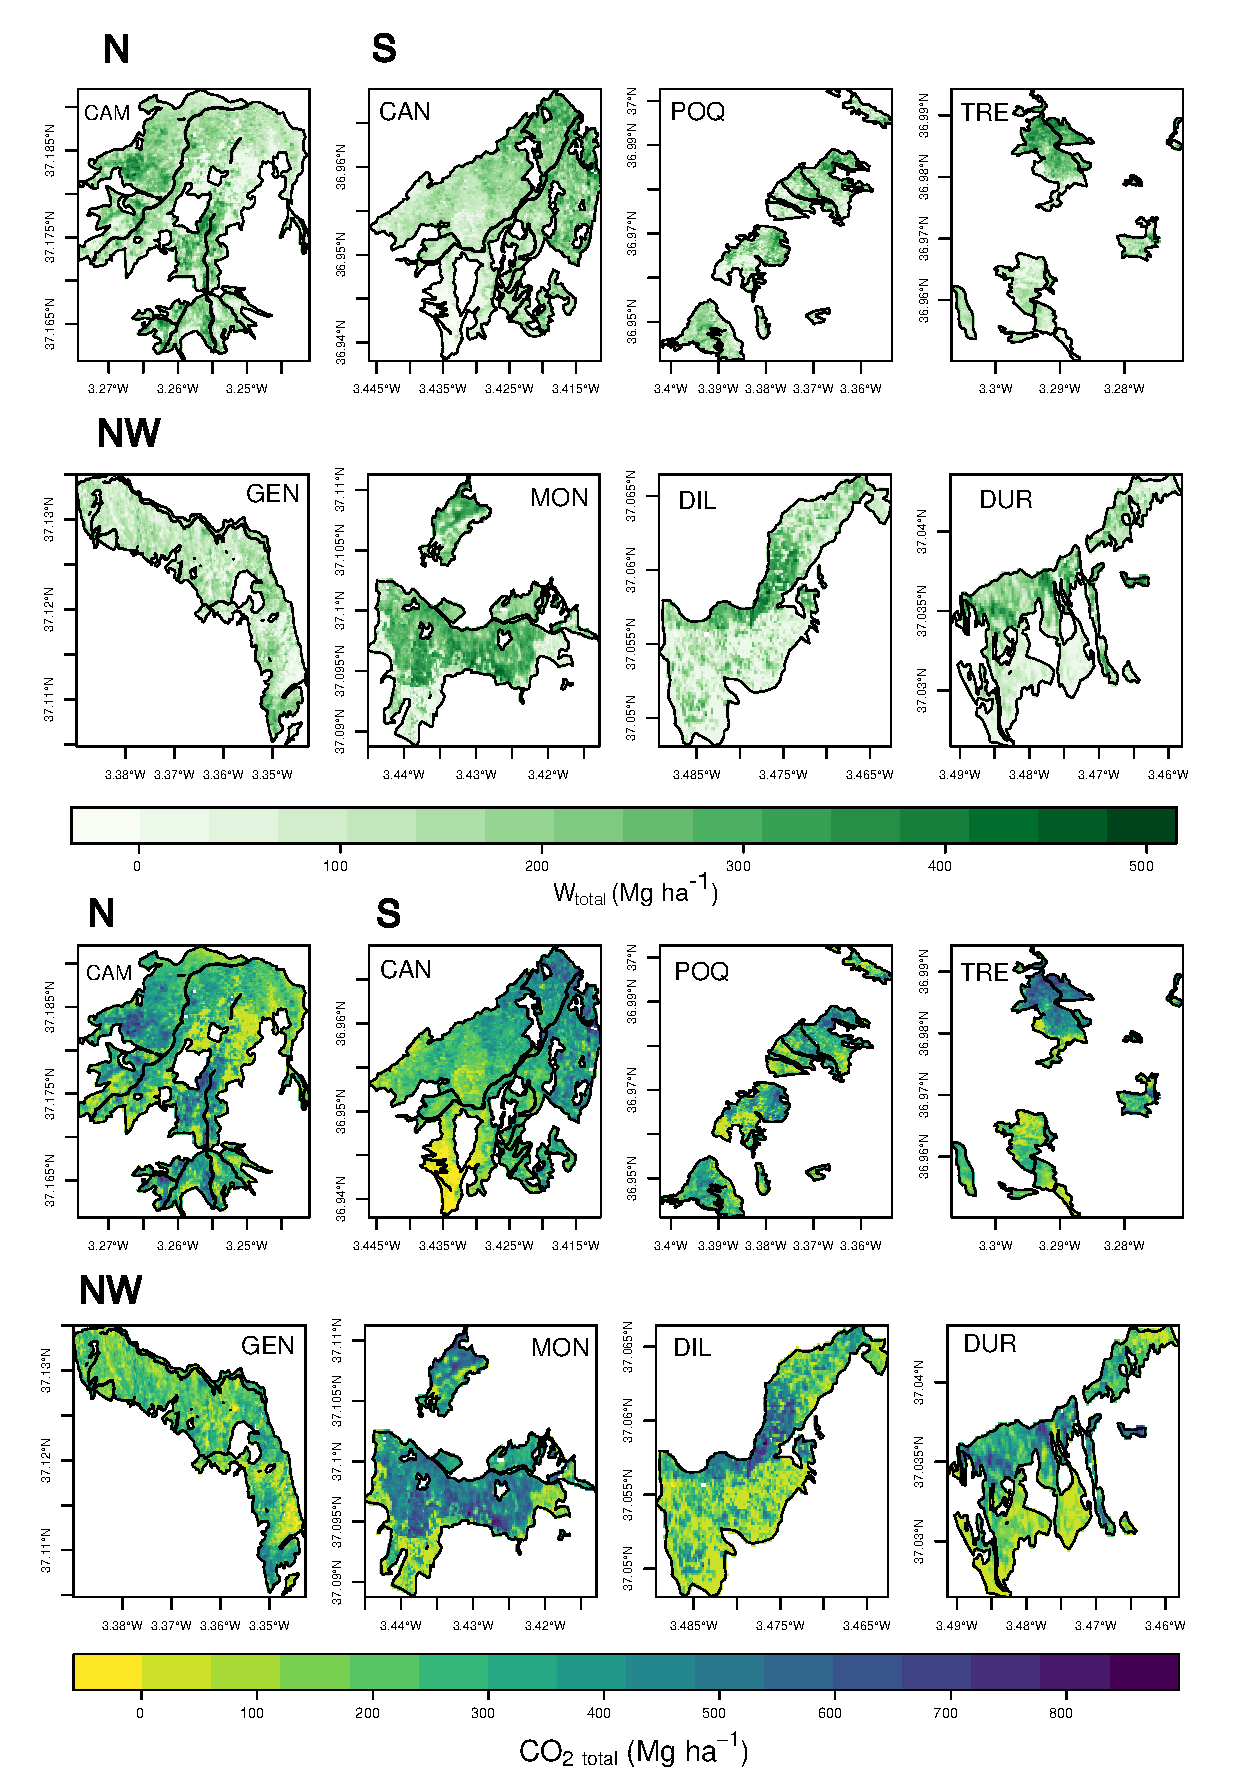
\includegraphics[width=\textwidth]{img/carbon/carbon-mapas-wt-ct.pdf}
    \caption{Total biomass (\wt) (\textbf{a}) and Potential Carbon sequestration (\textbf{b}) for each of the eight Pyrenean oak populations of Sierra Nevada. Different spatial scales were used for ease of visualization.}
    \label{fig:carbon:mapas-wt}
\end{figure}

The comparison of field-derived measures between oak-cluster populations revealed differences for tree height and DBH, but no for Basal Area and Tree density (\tabref{tab:carbon:compara}). The oak woodlands of N-cluster showed significantly taller trees with larger DBH than those of the NW and S (\tabref{tab:carbon:compara}, \figref{fig:carbon:schema}). Lower tree density and higher basal area were observed for N oak-woodlands, but the differences were not significant with the other oak-populations. No differences were found for field-biomass estimation between oak-populations (\tabref{tab:carbon:compara}).

\begin{sidewaystable} 
\caption{Summary of the best model (in terms of Bayesian Information Criterion) of total (\wt), stem (\ws), and root (\wro) biomass (\mgha) as a function of field-plot variables.}
\label{tab:carbon:bestmodels}
\begin{adjustbox}{width=\linewidth}
	\begin{threeparttable}
		\begin{tabular}{@{}l|crr|crr|crr@{}} \toprule
 & \textbf{\wt} &  &  & \textbf{\ws} &  &  & \textbf{\wro} &  &  \\ 
\textbf{\emph{Effects}} & \textbf{\emph{Estimate}} & \textbf{\emph{Z-value}} & \textbf{\emph{p-value}} & \textbf{\emph{Estimate}} & \textbf{\emph{Z-value}} & \textbf{\emph{p-value}} & \textbf{\emph{Estimate}} & \textbf{\emph{Z-value}} & \textbf{\emph{p-value}} \\ \toprule
Intercept & -1094.19 ± 292.09 & -3.75 & \textless{}0.001 & -721.44 ± 188.25 & -3.83 & \textless{}0.001 & -224.74 ± 68.09 & -3.3 & 0.001 \\
\textbf{$Ln$ Tree density (trees ha$^{-1}$)} & 102.04 ± 44.97 & 2.27 & 0.03 & 73.14 ± 28.98 & 2.52 & 0.01 & 22.08 ± 10.48 & 2.11 & 0.04 \\
\textbf{Elevation (m)} & 0.31 ± 0.05 & 6.77 & \textless{}0.001 & 0.17 ± 0.03 & 5.83 & \textless{}0.001 & 0.07 ± 0.01 & 6.83 & \textless{}0.001 \\
\textbf{Structural diversity index} & 2617.14 ± 828.65 & 3.16 & 0.002 & 1809.87 ± 534.06 & 3.39 & 0.001 & 542.41 ± 193.18 & 2.81 & 0.006 \\
\textbf{$Ln$ Tree density $\times$ Structural diversity index} & -349.22 ± 122.01 & -2.86 & 0.005 & -242.94 ± 78.63 & -3.09 & 0.003 & -76.26 ± 28.44 & -2.68 & 0.009 \\ \midrule
\textbf{Degree of freedom} & 101 &  &  & 101 &  &  & 101 &  &  \\
\textbf{AIC} & 1196 &  &  & 1103 &  &  & 887 &  &  \\
\textbf{BIC} & 1212 &  &  & 1119 &  &  & 903 &  &  \\
\textbf{Deviance Explained} & 0.413 &  &  & 0.373 &  &  & 0.381 &  &  \\ \bottomrule
\end{tabular}
\end{threeparttable}
\end{adjustbox}
\end{sidewaystable}

Significant differences for ALS-estimated biomass were found among oak-clusters (\tabref{tab:carbon:compara}). The values for the stem fraction (\ws) and small branches (\wb) biomass fractions were significantly higher for S oak-populations than for those in the N and NW, the latter showing no differences (\tabref{tab:carbon:compara}). The total biomass (\wt) was significantly different between oak-population clusters with higher values for southern oak populations (\figref{fig:carbon:schema}). Root biomass (\wro) and medium branches biomass (\wbs) were significantly higher for northern oak-populations (N) (\tabref{tab:carbon:compara}; \figref{fig:carbon:schema}).

\begin{figure}
    \centering
    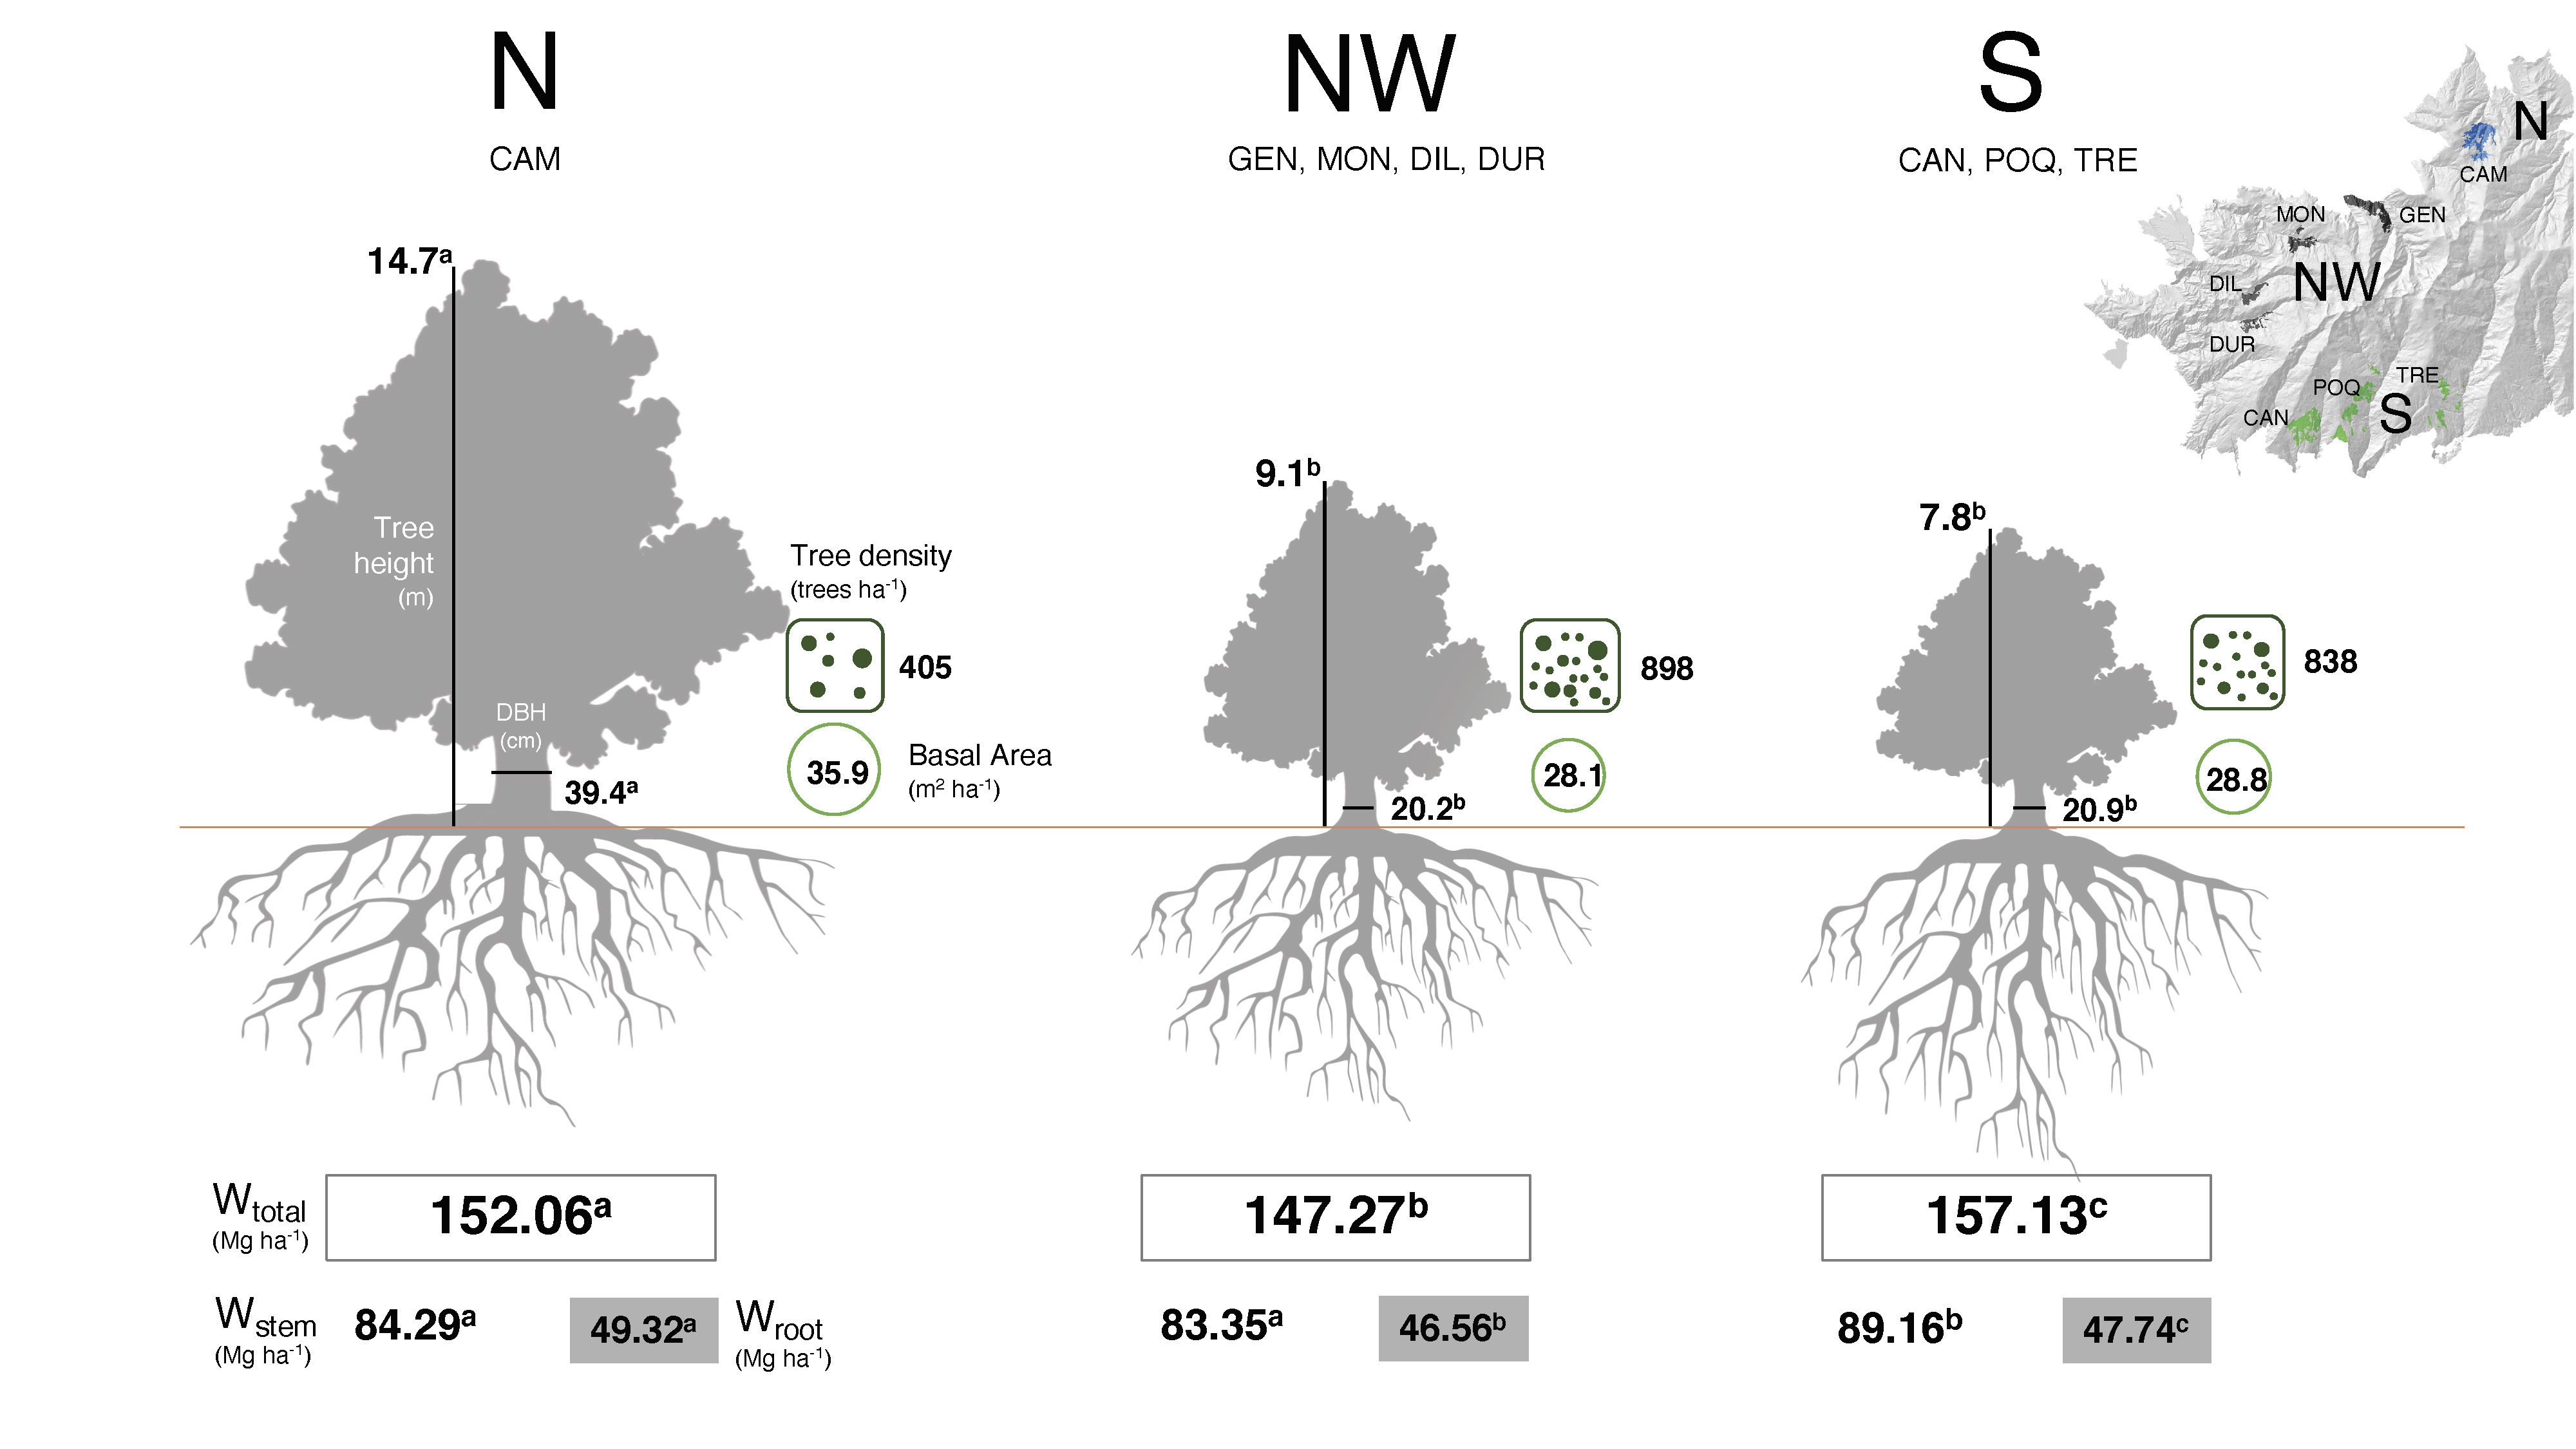
\includegraphics[width=\textwidth]{img/carbon/carbon-esquema-compara2.jpg}
    \caption{Comparison of stand features and ALS-estimated biomass fractions between oak-population clusters of \Qpy woodlands in Sierra Nevada. The distribution of oak-cluster are shown upper-right. Different letters indicate statistically significant differences between oak-population clusters (Dunn's test, p \textless 0.05) after Kruskal-Wallis test.}
    \label{fig:carbon:schema}
\end{figure}

\subsection{Predictions of Stand Biomass}\label{sec:carbon:results-prediction}
The best GLM models selected for total (\wt), stem (\ws) and root (\wro) biomass explained 70.3\%, 67.3\% and 63.1\% of variance respectively (\tabref{tab:carbon:bestmodels} and \tabref{tab:carbon:model-selection}). The elevation and the shannon structural diversity index showed positive effects on estimated biomass (\tabref{tab:carbon:bestmodels}; \figref{fig:carbon:glm}). Tree density negatively affected the estimated total biomass. The interaction between tree density and the shannon structural diversity index was significantly (\tabref{tab:carbon:bestmodels}), indicating that the total biomass increased with the increase structural diversity at lowest and medium tree densities, but decreased at high values of tree density (\figref{fig:carbon:glm}).

\begin{figure}
    \centering
    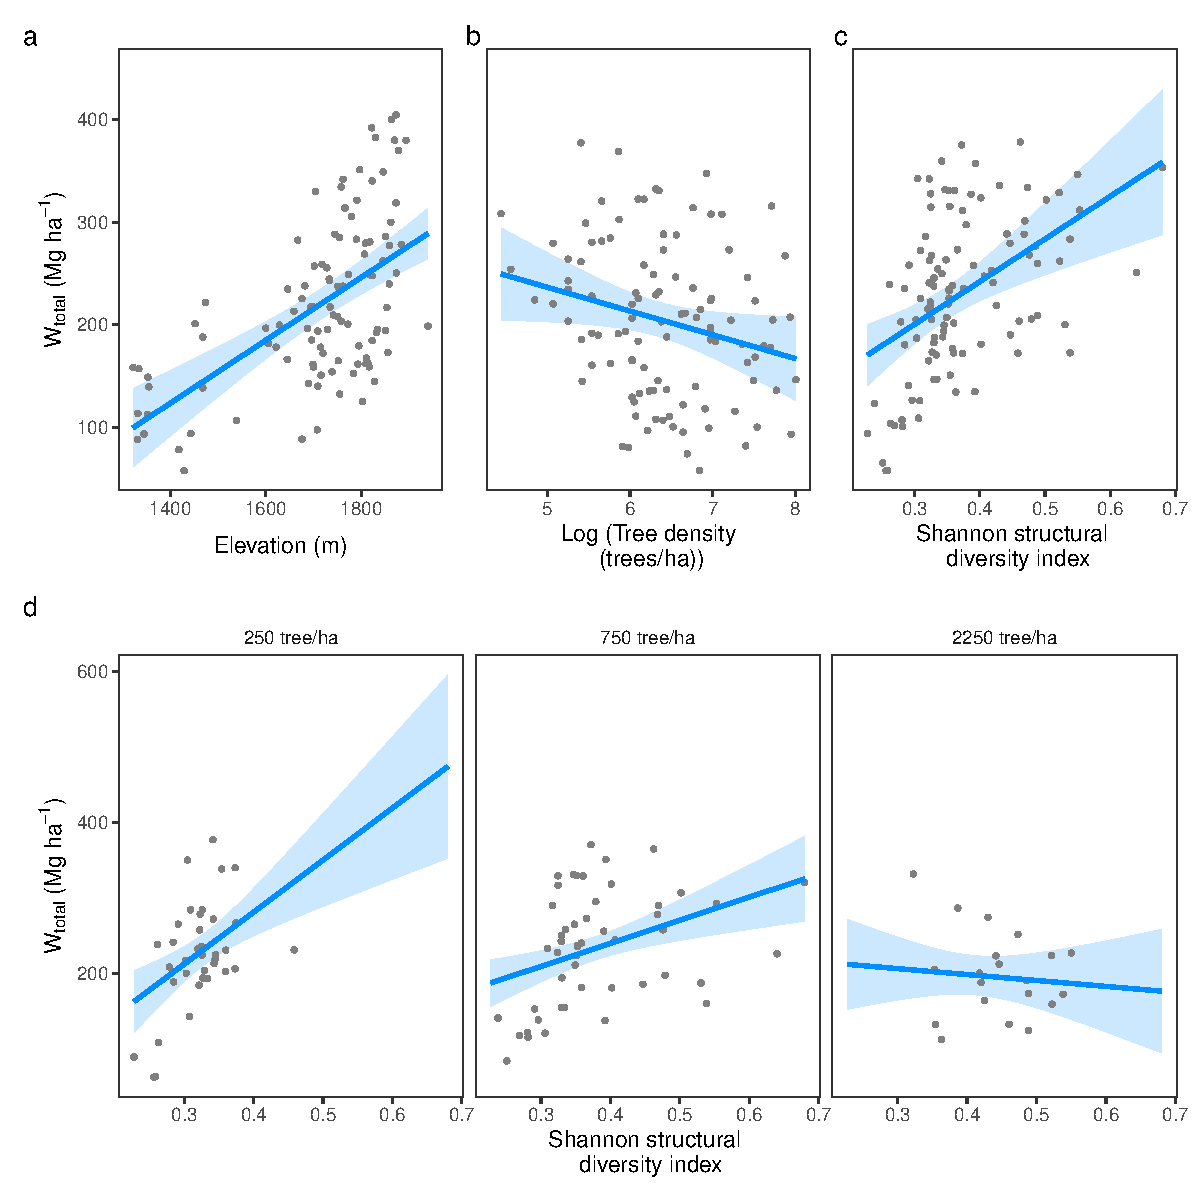
\includegraphics[width=\textwidth]{img/carbon/carbon-glm-effects.pdf}
    \caption{Predicted effects of the (\textbf{a}) elevation (meters), (\textbf{a}) tree density (trees ha\textsuperscript{-1}), (\textbf{c}) shannon structural diversity index, and (\textbf{d}) tree density $\times$ shannon structural diversity index, on the total biomass (\wt; \mgha).}
    \label{fig:carbon:glm}
\end{figure}


\subsection{Temporal evolution of Biomass in \Qp stands}\label{sec:carbon:results-temporal}
A general pattern of increase in aboveground tree biomass was observed for most analyzed plots (\tabref{tab:carbon:temporal}), with a total increase of 19 172 \mgha between the two national forest inventories. About 89 \% of the plots showed an increase in aboveground tree biomass, with an average of 11.46 \mgha (\tabref{tab:carbon:temporal}). This general pattern was also observed for plots located in Sierra Nevada (\figref{fig:carbon:ifn}).

\begin{figure}
    \centering
    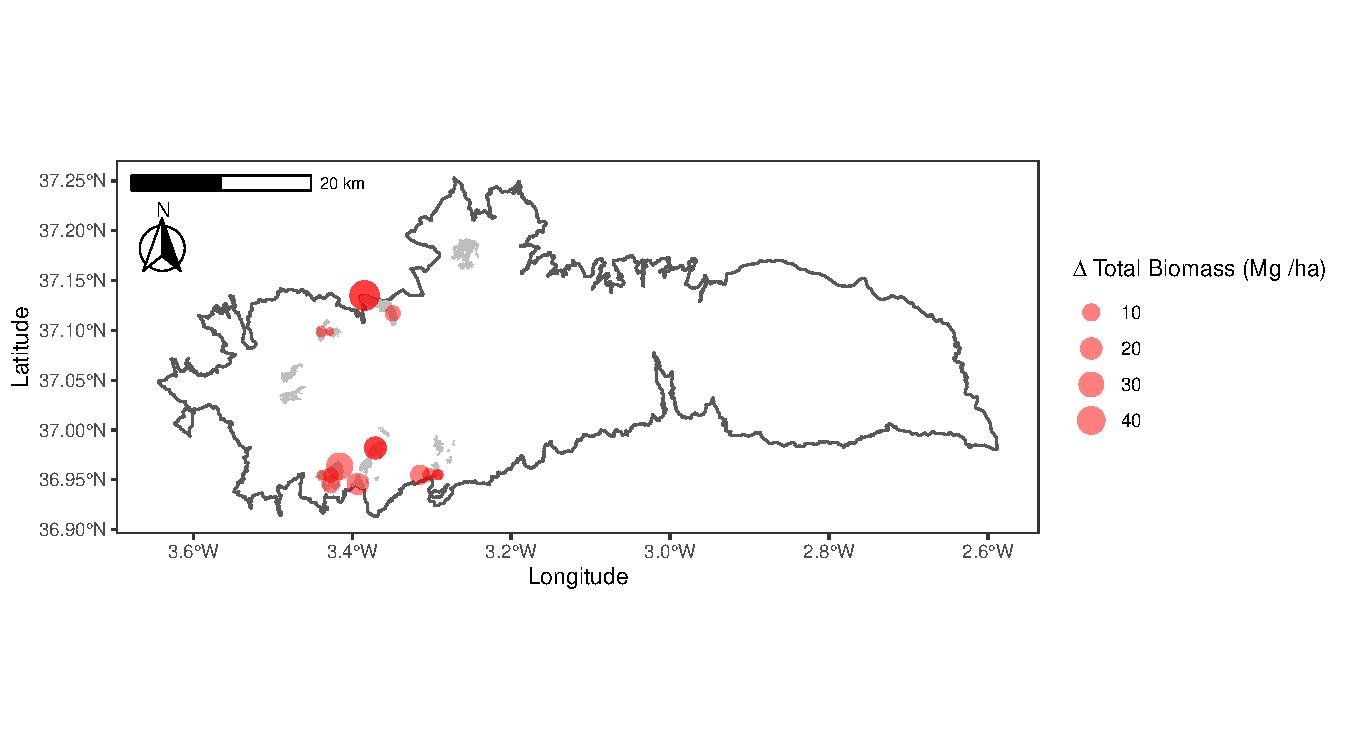
\includegraphics[width=\textwidth]{img/carbon/carbon-mapa-ifn.pdf}
    \caption{Variation of tree biomass between the second and third Spanish National Forest Inventories, for plots (points) located on Sierra Nevada which have \Qp as the main species. Size point indicates the variation in total biomass ($\Delta$ \mgha).}
    \label{fig:carbon:ifn}
\end{figure}

\begin{table}[]
\caption{Temporal evolution of the total biomass (\mgha) of \Qp and the total carbon (\mgha) between the second (SNFI2) and third (SNFI3) Spanish National Forest Inventories. Plots were aggregated by loss/gains of the tree numbers ($\Delta$ trees), and also by increase/decrease of biomass during the period analyzed. The total variation in biomass (\emph{i.e.} sum for all plots), and the average variation per plot are shown for each category. }
\footnotesize
\label{tab:carbon:temporal}
\resizebox{\textwidth}{!}{%
\begin{tabular}{clc|>{\centering}p{2cm}|>{\centering}p{3cm}|c}
\toprule
$\Delta$ \textbf{trees} & \textbf{Biomass} & \textbf{\# plots} & $\Delta$ \textbf{total biomass (\mgha)} & \textbf{Average  variation per plot (\mgha)} & \textbf{ Total Carbon} \tabularnewline \toprule
\multirow{2}{*}{\textless 0} & Decrease & 159 & -1060.39 & -6.67 (0.86) & -1846.85 \tabularnewline
 & Increase & 123 & 921.40 & 7.49 (0.86) & 1604.77 \tabularnewline \midrule
\multirow{2}{*}{\textgreater 0} & Decrease & 33 & -287.19 & -8.7 (2.82) & -500.19 \tabularnewline
 & Increase & 1586 & 18183.25 & 11.46 (0.41) & 31669.16 \tabularnewline \midrule
\multirow{2}{*}{0} & Decrease & 56 & -141.40 & -2.53 (0.59) & -246.28 \tabularnewline
 & Increase & 312 & 1556.16 & 4.99 (0.48) & 2710.32 \tabularnewline
 \bottomrule
\end{tabular}%
}
\end{table} 
\normalsize

\section{Discussion}\label{sec:carbon:discussion}
\section{Carbon sequestration by Sierra Nevada oak woodlands.}\label{sec:carbon:discussion-sn}

Total estimated biomass values in Sierra Nevada oak woodlands ranged from 147.27 -- 157.13 \mgha (\tabref{tab:carbon:compara}), with aboveground biomass (sum of \ws, \wb and \wbs fractions) ranging from 104.69 - 111.71 \mgha. Our results are consistent with the mean aboveground biomass density cited by the IPCC guidelines as the default value for temperate mountain systems (130 (20 - 600) \mgha) in Europe \autocite{IPCC2006ForestLand}. Using data from the Spanish Third National Forest Inventory, \citet{Vayredaetal2012SpatialPatterns} reported an average value for stand C stock of 45 \mgha along the distribution of \Qp in the Iberian Peninsula. Those values were lower than the estimated carbon stock (above- and below-ground) in our study which ranged from 69.95 - 74.63 \mgha (\tabref{tab:carbon:compara}). At a more regional scale, our results showed higher values than those found in the central range of the species distribution, where aboveground biomass varied between 63.8 - 98 \mgha \autocite{GallardoLanchoGonzalezHernandez2004SequestrationCarbon}. Estimates of dioxide carbon sequestration for \Qp pure stands (122.19 - 152.82 \mgha) located in the Central Mountain Range (Spain) \autocite{Canellasetal2008SilvicultureCarbon,Canellasetal2017CarbonSequestration} were also lower than our results (256.72 - 273.91) (\tabref{tab:carbon:compara}). Despite the potential differences derived from the carbon estimation method (\emph{i.e.} LIDAR estimation \emph{versus} field-ground based estimation; biomass expansion factors), several factors could explain the differences found in our results with respect to the values reported for other studies. First, it is generally accepted that there is an age‐related decline in stand biomass accumulation \autocite[ and references therein]{Xuetal2012AgerelatedDecline} with the productivity of old-growth forests being usually lower than younger forests \autocite{Kutschetal2009EcophysiologicalCharacteristics}. Oak woodlands of Sierra Nevada are composed of relatively young trees \autocite{GeaIzquierdoCanellas2014LocalClimate,PerezLuqueetal2020LanduseLegacies,RubioCuadradoetal2018AbioticFactors} in comparison with other woodlands of the species along their distribution area \autocite{GeaIzquierdoCanellas2014LocalClimate}. The strong anthropic perturbations in these oak has conditioned their structure. For instance, some of the oak woodlands were massively cut down during Spanish Civil post-war period for use as wood gas for vehicles \autocite[\emph{e.g.} MON population;][]{Prieto1975BosquesSierra}, or for use in intense mining activities \autocite[\emph{e.g.} GEN population;][]{PerezLuqueetal2020LanduseLegacies}. Therefore, we can consider that many of the oak woodlands of Sierra Nevada oaks are relatively young, which might explain the high potential for C accumulation obtained in our study, since it has been shown that forest created as a result of drastic land-use changes exhibited faster growing rates, and therefore higher potential C accumulation, than pre-existing forests \autocite{VilaCabreraetal2017NewForests}. Differences in carbon stock between young oak coppices and mature forests were reported for other \emph{Quercus} species \autocite{Bruckmanetal2011CarbonPools,Cotillasetal2016AbovegroundBelowground}. Therefore, it is likely that the high total ecosystem C values obtained in our area of study could be partly explained by the stands age-development stage \autocite{Makinecietal2015EcosystemCarbon}. Secondly, the water availability is generally the most limiting factor driving radial growth of \Qp along its distribution range in the Iberian Peninsula \autocite{GeaIzquierdoCanellas2014LocalClimate}. In Sierra Nevada, northern and northwestern oak populations are located in valley bottoms with high values of relative humidity; and southern ones get the extra supply of water from moist air from the Mediterranean sea. Therefore water availability does not seem to be strongly limiting the oak-growth in this mountain region. In fact, in the last decades positive trends have been observed for greenness and secondary growth of oak woodlands in Sierra Nevada \autocite{GeaIzquierdoCanellas2014LocalClimate,PerezLuqueetal2020LanduseLegacies,RubioCuadradoetal2018AbioticFactors} suggesting that this mountain range could act as an ecological refugee for this species. Thus those positive growth trends could explain the high values of carbon sequestration obtained in our study.

\subsection{Factors explaining biomass in the oak woodlands}\label{sec:carbon:discussion-factors}
Regarding the factors explaining biomass, we found a positive effect of the structural richness on total biomass, and therefore on C stock (\figref{fig:carbon:glm}). Our results are consistent with general patterns obtained for tree species in Iberian Peninsula \autocite{Vayredaetal2012SpatialPatterns}. In structural-heterogeneous stands, trees occupy different horizontal and vertical layers, thus they can maximize the resources \autocite[\emph{e.g.} light][]{Forrester2014StandlevelLight}, whereas homogeneous stand structure may reduce complementary effects \autocite{Goncalves2018EffectsForest,Vayredaetal2012SpatialPatterns}. Being surrounded by size-diverse neighbours allow trees to fill the available canopy space around them and hence capture more light \autocite{Forrester2014StandlevelLight,Vanhellemontetal2018SpeciesStructural}. Our results show that the higher the tree density, the lower the total biomass (\figref{fig:carbon:glm}).
Previous studies on forests located on NW of Spain, reported tree stand density as one of the main factors affecting potential biomass production and carbon sequestration \autocite{CastanoSantamariaetal2013PotentialGround}. Tree growth of \Qp is inversely influenced by competition \autocite{Canellasetal2004GrowthResponse,FernandezdeUnaetal2015StandCompetition,FernandezdeUnaetal2016DisentanglingEffect}. Thus, trees respond to reduced competition through the structural shifts such as increased radial growth \autocite{Canellasetal2004GrowthResponse,FernandezdeUnaetal2016DisentanglingEffect}, and therefore a potential increase in biomass. We also found an interaction effect between the tree-density and stand structure diversity (\figref{fig:carbon:glm}) which suggests that at high tree-densities resources are not maximized, even if structural diversity exists.
Despite the importance of the water availability in the growth of \Qp \autocite{GeaIzquierdoCanellas2014LocalClimate,MorenoFernandezetal2020InfluenceClimate}, none of the best models selected for \wt, \ws or \wro, included the topographic wetness index (\tabref{tab:carbon:model-selection}). This would seem suggest that the water requirement of this species in this mountain is met by the location of the oak populations within Sierra Nevada, and therefore would reinforce the role of this mountain region as an ecological refugee for this species.

\subsection{Biomass differences within oak woodlands}\label{sec:carbon:discussion-differences}
We found that oak woodlands of the Northern cluster showed stands with taller and greater trees (\tabref{tab:carbon:compara}), and also high values of biomass (Figures \ref{fig:carbon:mapas-wt} and \ref{fig:carbon:schema}). It could be related with lower intensity of anthropogenic disturbances in comparison with the other oak woodlands, mainly because the northern oak woodlands had greater protection during the second half of the last century \autocite{JimenezOlivencia1991PaisajesSierra}, and currently also have the highest level of legal protection within the protected area \autocite{Anonymous2011Decreto238}. The less anthropogenic disturbances have resulted in well-conserved forests with a greater species diversity \autocite{PerezLuqueetal2021EcologicalDiversity}, and also a stable stand structure with high values of biomass (Figures \ref{fig:carbon:mapas-wt} and \ref{fig:carbon:schema}). For other species of \emph{Quercus} it has been observed that forests with less disturbance have a higher potential for carbon storage \autocite{BalboaMuriasetal2006CarbonNutrient,Cotillasetal2016AbovegroundBelowground,Stojanovicetal2017ForecastingTree}.

Our results also highlighted how differences in stand structure conditioned stand tree biomass (\tabref{tab:carbon:bestmodels}, \figref{fig:carbon:glm}). High dense stands, \emph{i.e.} northwestern oak populations, showed lower total biomass than less dense stands (northern or southern oak populations) (\figref{fig:carbon:schema}). High stand density increase tree competition, limiting stand growth which provokes loss of vitality and reduction in acorn production \autocite{Bravoetal2008SelviculturaMontes,Piqueetal2018Spain}, and according to our results, the higher the tree density the lower the capacity of these forests to act as carbon sinks (Figures \ref{fig:carbon:schema}, \ref{fig:carbon:glm}). In addition, an accumulation of biomass, coupled with a loss of structural diversity (\figref{fig:carbon:glm}), would increase the risk of forest fires due to the large amount of biomass \autocite{Canellasetal2004GrowthResponse,PiqueVericat2015EvolutionPerspectives,Serradaetal1992CoppiceSystem}

\subsection{Trends of carbon sequestration by oak woodlands}\label{sec:carbon:discussion-trends}
We observed an increase in aboveground tree biomass between the two inventories for plots located in oak woodlands (\tabref{tab:carbon:temporal}, \figref{fig:carbon:ifn}). Recent studies have reported a positive trend for primary production and for secondary growth in oak woodlands in Sierra Nevada \autocite{AlcarazSeguraetal2016ChangesVegetation,Dionisioetal2012SatelliteBasedMonitoring,PerezLuqueetal2015OntologicalSystem,PerezLuqueetal2020LanduseLegacies}. In addition, an increase in the area occupied by oak forests \autocite{CamachoOlmedoetal2002TransformacionPaisaje} as well as the densification of existing forest have been found \autocite{JimenezOlivenciaetal2015MedioSiglo}. All these results indicated that this ecosystem service, \emph{i.e.} carbon sequestration, have suffered an increase in the last decades in our study area. Land-use changes have extensively affected C storage of terrestrial ecosystems for several areas of south Europe \autocite{MunozRojasetal2011ChangesLand,MunozRojasetal2015ImpactLand}. Abandonment of traditional activities and rural exodus are the main drivers explaining the densification and expansion of forests particularly in mountainous regions such as Sierra Nevada \autocite{JimenezOlivenciaetal2015MedioSiglo,MacDonaldetal2000AgriculturalAbandonment}. Considering the positive trend observed for the increase in biomass, and the lack of direct human-drive disturbances as these forests are in a protected area, it would expect a positive trend in forest carbon stock, such as has been recorded in many forests in the Mediterranean region in the last decades \autocite{FAOPlanBleu2018StateMediterranean}. It also agrees with the predictions under different scenarios forecasting a forest growth in the next decades \autocite{Aparicioetal2015ClimateChange}. However, it should be taken with caution, since some early signs of saturation of forests as a carbon sink are being documented in Europe \autocite{Nabuursetal2013FirstSigns}.

\section{Management implications}\label{sec:carbon:discussion-management}

Several studies indicated that reductions of tree-density on oak coppices forests, by moderate thinning, causes an increase in the tree growth and biomass for \Qp woodlands \autocite{Aldeaetal2017ThinningEnhances,Aldeaetal2017EfectoClaras,MorenoFernandezetal2020InfluenceClimate,Canellasetal2004GrowthResponse}, and also for other \emph{Quercus} species \autocites[\emph{e.g.}][]{Cotillasetal2009GrowthResponse,FernandezdeUnaetal2015StandCompetition}. This reduction in the stand density could increase the carbon sequestration of the woodland by a higher structural diversity which maximized the use of resources \autocite{CastanoSantamariaetal2013PotentialGround}. Esta reducción de la densidad, además implica una menor cantidad de biomasa de pequeño tamaño, mejorando las condición fuegos